\section{Results}
\label{sec:results}

\subsection{Zero-shot screening and finalist reruns}

The internal-dev screening matrix immediately separates backbone quality from prompt sensitivity. Figure~\ref{fig:screening-heatmap} shows that Qwen2.5-VL-3B dominates the full screening stage, with its best configuration (\texttt{short\_answer}) reaching 81.05\% accuracy and its weakest OCR-heavy variant still remaining competitive. The ranking is not a trivial prompt artifact: even after allowing six prompt/OCR settings per backbone, Qwen remains clearly ahead of LLaVA-Phi-3-mini, BLIP-2 OPT-2.7B, InternVL2.5-4B, and the OCR lexical baseline. The same figure also shows that prompt sensitivity is model dependent. Qwen prefers concise answer formatting, whereas LLaVA benefits more from OCR-normalized prompting; by contrast, BLIP-2 remains weak across all prompt variants, and InternVL2.5-4B never becomes competitive under the study protocol.

\begin{figure*}[t]
    \centering
    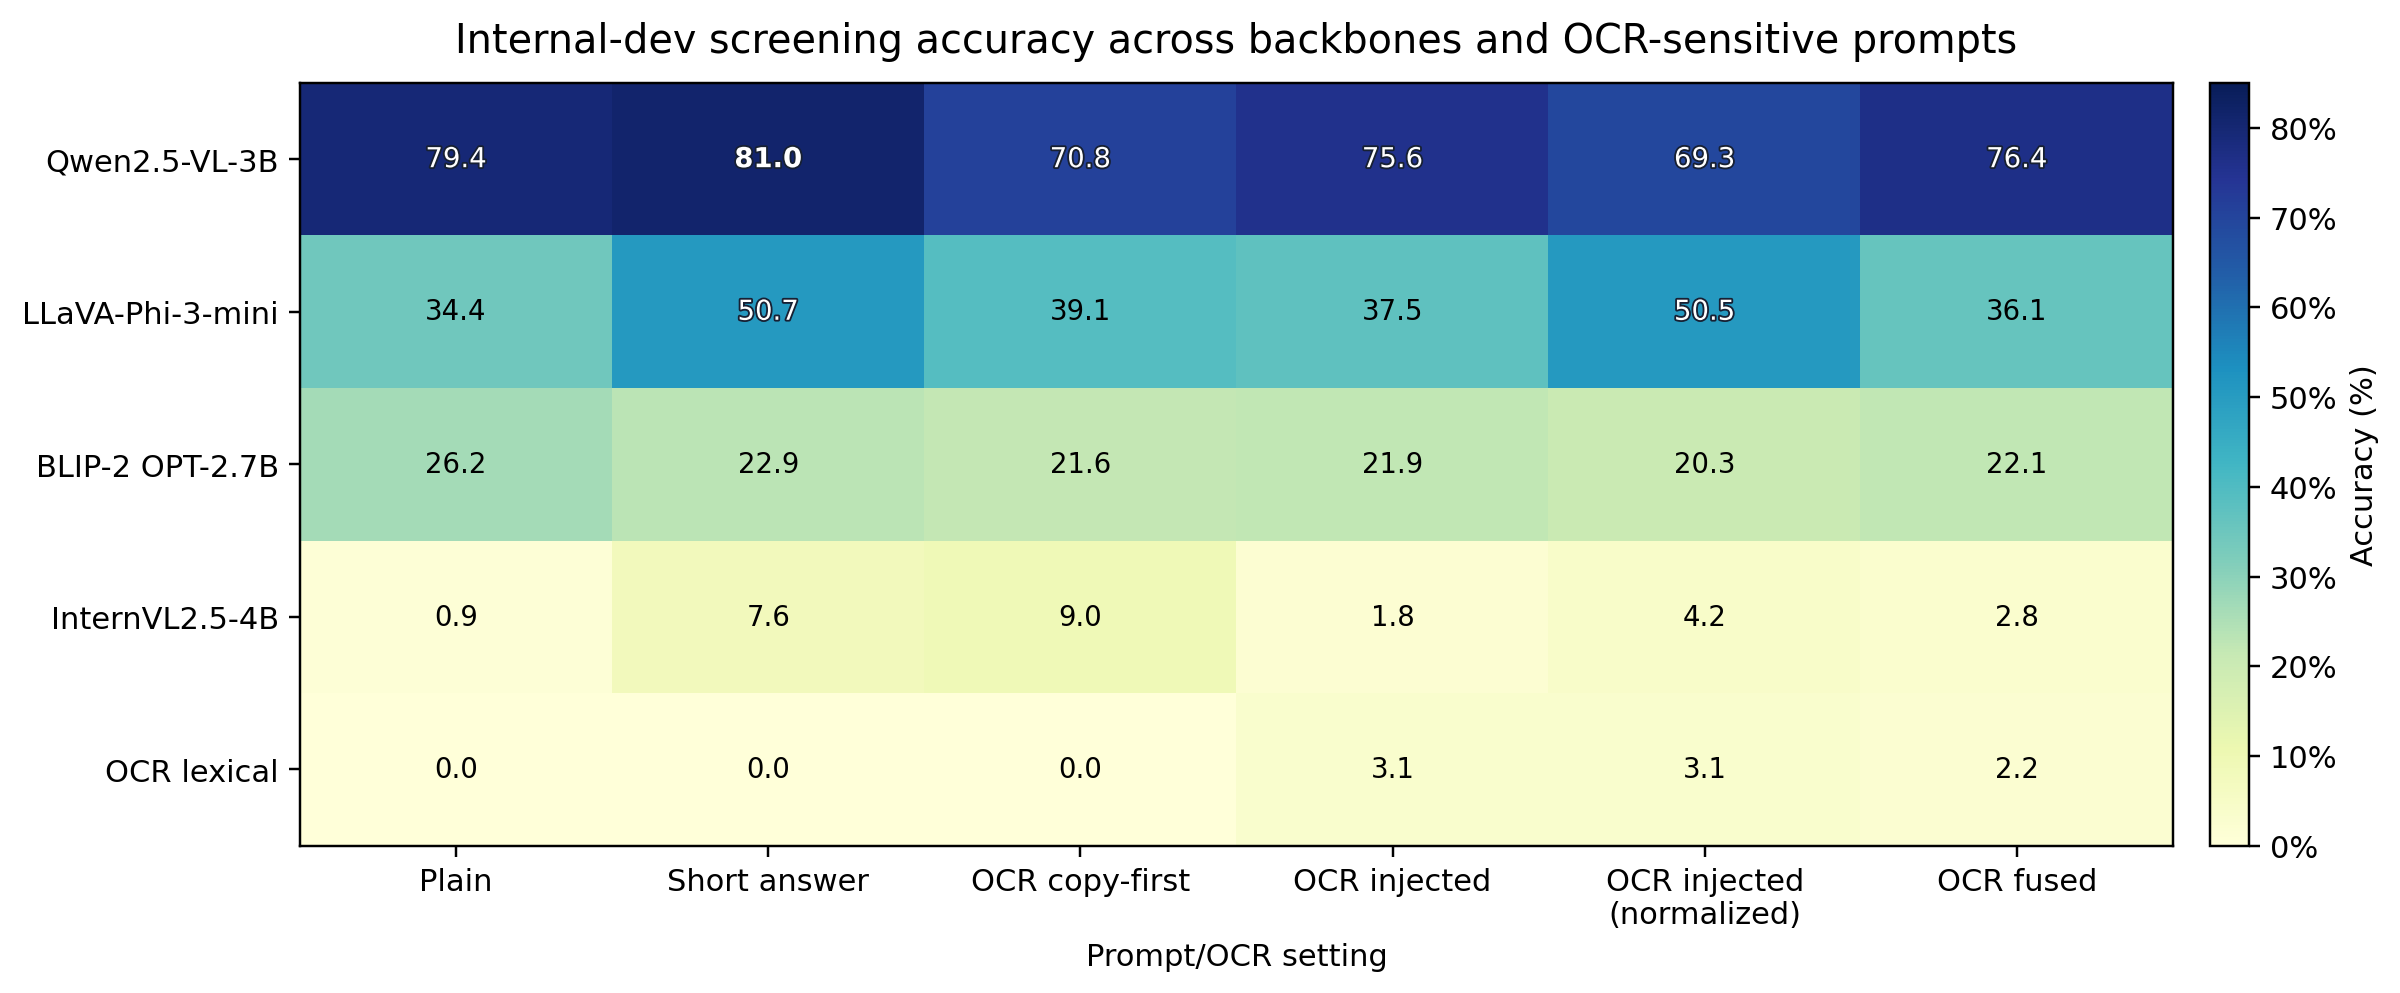
\includegraphics[width=\textwidth]{figures/screening_heatmap.png}
    \caption{Internal-dev screening accuracy across the full backbone--prompt matrix. Qwen2.5-VL-3B is the only family that remains strong across all OCR-sensitive prompt variants, and its short-answer prompt is the best zero-shot configuration overall. The heatmap also makes the model-dependent nature of OCR prompting visible: OCR normalization helps LLaVA markedly more than it helps Qwen, while the lexical OCR baseline remains near zero throughout.}
    \label{fig:screening-heatmap}
\end{figure*}

The finalist stage confirms that the screening winner transfers to the official validation split. Table~\ref{tab:main-results} shows that the four promoted Qwen settings occupy the top four validation positions, led again by \texttt{short\_answer} at 78.72\% accuracy and 89.09\% judge similarity. The strongest non-Qwen finalist, LLaVA-Phi-3-mini with OCR-normalized prompting, reaches only 50.36\% exact-match accuracy, leaving a 28.36-point gap to the best Qwen finalist. This margin is large relative to the within-family prompt differences, so under the current evaluation boundary the main zero-shot ranking is better explained by backbone quality than by any single OCR-aware prompt variant.

\begin{table*}[t]
    \centering
    \small
    \resizebox{\textwidth}{!}{\begin{tabular}{llcccccc}
\toprule
Stage & Model / setting & Acc. & Cons. & F1 & BLEU & METEOR & ROUGE-L\\
\midrule
Best screening & Qwen2.5-VL-3B (short answer) & 81.05 & 77.20 & 70.24 & 13.48 & 51.26 & 72.38\\
Best screening & LLaVA-Phi-3-mini (short answer) & 50.70 & 46.93 & 45.74 & 7.29 & 36.24 & 48.03\\
Best screening & BLIP-2 OPT-2.7B (plain) & 26.25 & 23.50 & 23.62 & 2.58 & 25.13 & 24.83\\
Best screening & InternVL2.5-4B (ocr copy first) & 9.05 & 8.78 & 11.84 & 0.14 & 8.26 & 19.77\\
Best screening & OCR lexical (ocr injected) & 3.15 & 2.83 & 10.45 & 0.59 & 11.00 & 11.43\\
Finalist & Qwen2.5-VL-3B (short answer) & 78.72 & 74.45 & 70.42 & 14.88 & 48.08 & 73.45\\
Finalist & Qwen2.5-VL-3B (plain) & 77.18 & 72.91 & 69.47 & 14.64 & 47.81 & 72.78\\
Finalist & Qwen2.5-VL-3B (ocr fused) & 75.56 & 70.93 & 67.37 & 14.14 & 46.88 & 70.84\\
Finalist & Qwen2.5-VL-3B (ocr injected) & 74.42 & 69.99 & 66.69 & 13.92 & 45.93 & 70.26\\
Finalist & LLaVA-Phi-3-mini (ocr injected normalized) & 50.36 & 46.98 & 48.72 & 7.26 & 35.49 & 52.34\\
Finalist & LLaVA-Phi-3-mini (short answer) & 46.70 & 43.42 & 45.08 & 7.68 & 33.06 & 47.99\\
Finalist & LLaVA-Phi-3-mini (ocr injected) & 40.68 & 37.65 & 41.66 & 5.13 & 32.26 & 46.80\\
Finalist & LLaVA-Phi-3-mini (ocr copy first) & 36.86 & 34.42 & 41.81 & 7.07 & 32.97 & 44.67\\
Tuned winner & Qwen2.5-VL-3B + LoRA (all-linear r16 seed13) & 84.76 & 80.39 & 74.92 & 14.26 & 50.66 & 77.56\\
\bottomrule
\end{tabular}
}
    \caption{Main benchmark results. The table reports the best internal-dev screening configuration for each backbone, all promoted validation finalists, and the final tuned model. Exact-match accuracy is the primary score; consensus accuracy, F1, BLEU, METEOR, ROUGE-L, and judge similarity provide secondary semantic context. The tuned Qwen adapter becomes the strongest overall validation system.}
    \label{tab:main-results}
\end{table*}

\subsection{Winner-conditioned LoRA adaptation}

The adaptation stage improves the official validation result, not only the internal diagnostic split. Figure~\ref{fig:adaptation-summary} reports the headline comparison: the final tuned model, \texttt{all-linear-r16-seed13}, reaches 84.76\% validation accuracy, compared with 78.72\% for the strongest zero-shot finalist, for an absolute improvement of 6.04 points. The same comparison also improves consensus accuracy by 5.95 points, F1 by 4.50 points, and ROUGE-L by 4.11 points. Because both systems are evaluated on the same 5,000 validation questions, we also run a paired bootstrap over examples. The paired 95\% confidence interval for the accuracy gain is $[5.00, 7.04]$ points, and an exact McNemar test on the discordant decisions gives $p=1.97\times10^{-32}$.

\begin{table}[t]
    \centering
    \small
    \begin{tabular}{lccc}
\toprule
System & Acc. [95\% CI] & Cons. & Judge\\
\midrule
Zero-shot Qwen finalist & 78.72 [77.60, 79.88] & 74.45 & 89.09\\
Tuned Qwen LoRA & 84.76 [83.86, 85.76] & 80.39 & 91.24\\
\midrule
Paired gain & 6.04 [5.00, 7.04] & -- & --\\
\bottomrule
\end{tabular}

    \caption{Official validation headline comparison. The paired gain is computed over the same 5,000 validation questions and is therefore a stronger test than comparing independent intervals alone.}
    \label{tab:validation-headline}
\end{table}

The semantic judge agrees with the direction of the exact-match result while tightening its interpretation. In Table~\ref{tab:main-results}, the strongest zero-shot finalist reaches 89.09\% judge similarity, whereas the tuned winner reaches 91.24\%, a gain of 2.15 points. This gap is smaller than the exact-match improvement, which is exactly the pattern we would expect if part of the tuned model's advantage comes from stricter normalization and answer-format control rather than from a wholesale change in semantic competence. In other words, the judge score does not erase the tuning gain; it refines it into a more conservative but still positive semantic improvement.

The internal-dev adapter sweep in Figure~\ref{fig:adaptation-summary} and Table~\ref{tab:trained-adapters} also reveals why the selection policy separates training loss from answer accuracy. Mean internal-dev \texttt{eval\_loss} selected the \texttt{all-linear-r32} family for the follow-up OCR and scaling diagnostics, but the highest post-train internal-dev answer accuracy among the completed core adapters came from \texttt{all-linear-r16-seed13} at 88.45\%. This is not a conflict between two winners; it is a distinction between two roles. Loss is used to allocate limited follow-up training budget, while answer accuracy selects the adapter promoted to official validation.

\begin{figure*}[t]
    \centering
    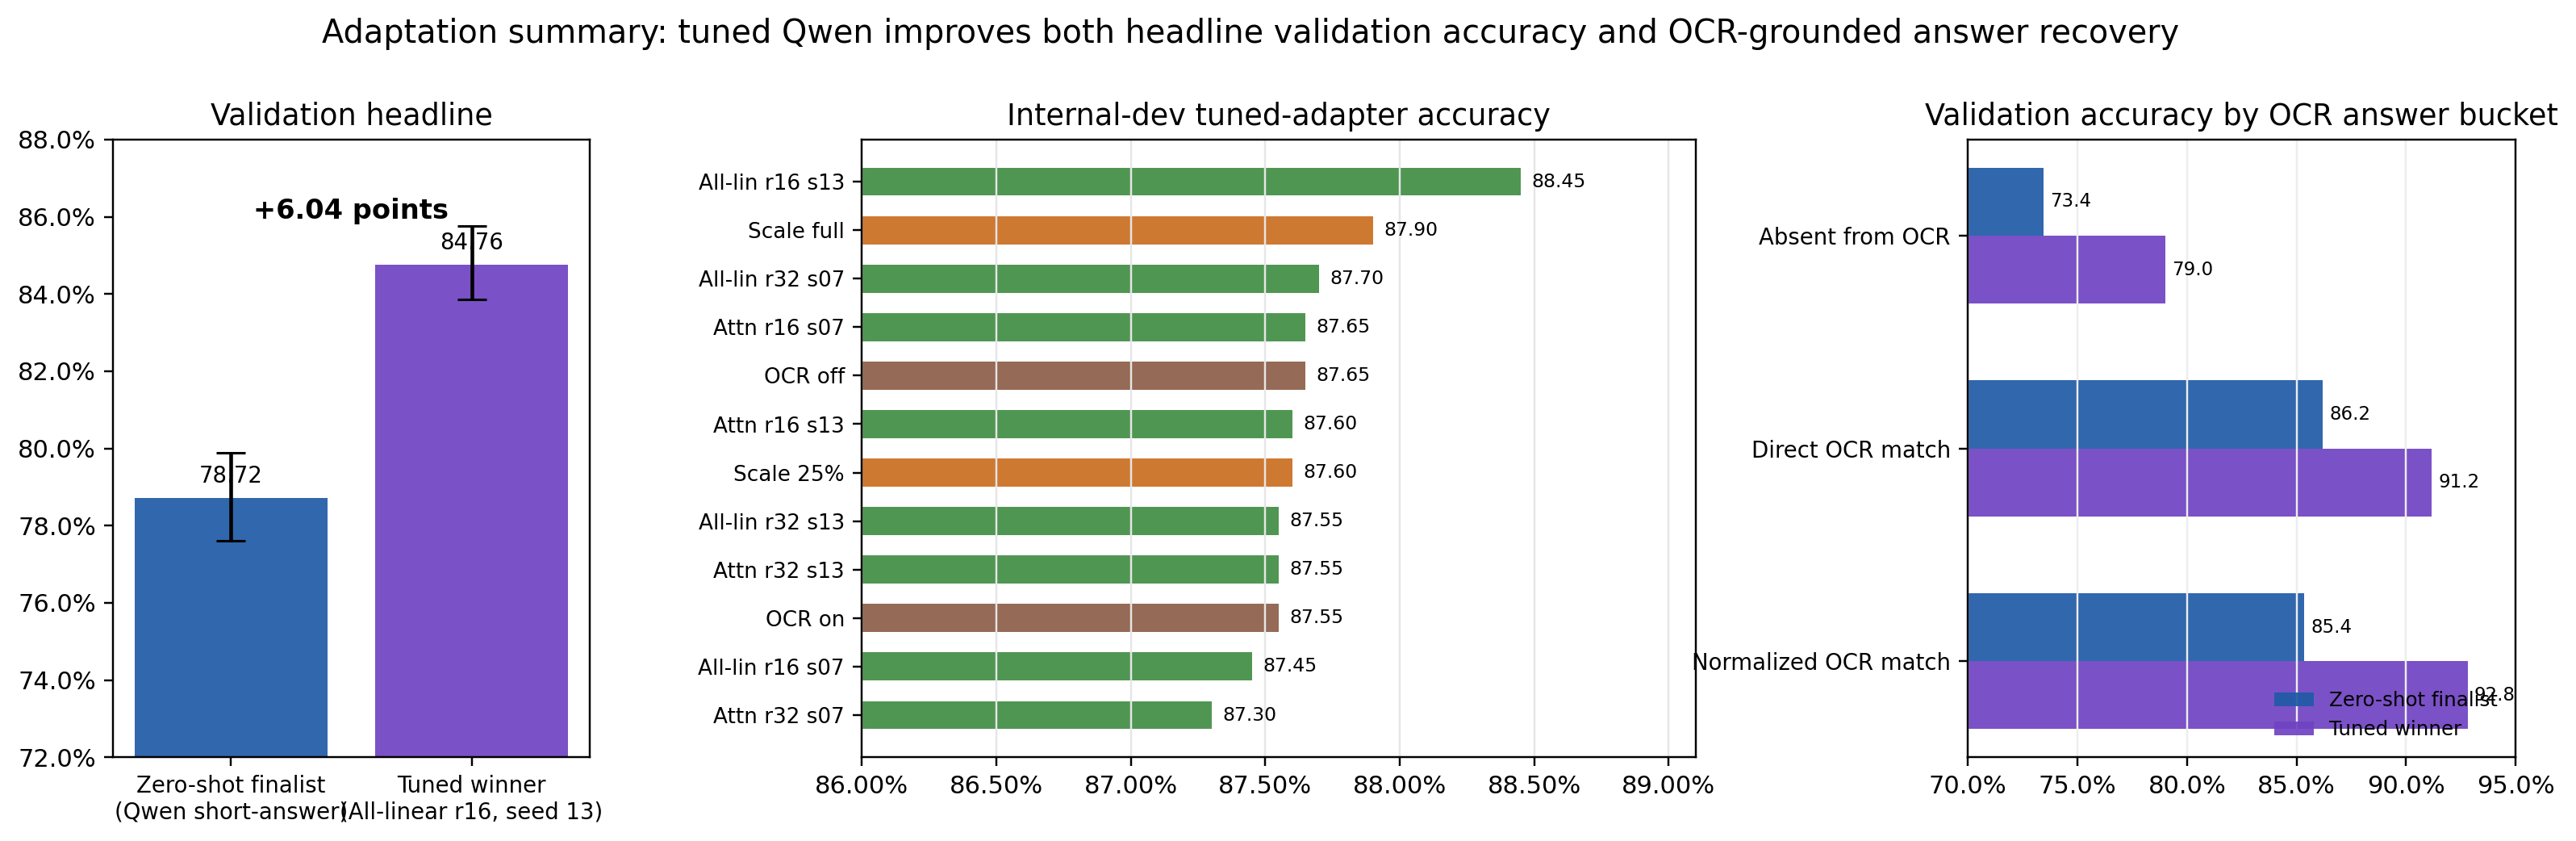
\includegraphics[width=\textwidth]{figures/adaptation_summary.png}
    \caption{Adaptation summary. Left: the final tuned Qwen model improves validation accuracy by 6.04 points over the strongest zero-shot finalist. Middle: internal-dev post-train accuracy across the full 12-run LoRA study, including the core matrix and winner-conditioned follow-ups. Right: validation gains are largest for OCR-grounded answers, especially those that require normalized OCR matching.}
    \label{fig:adaptation-summary}
\end{figure*}

Seed stability in the core matrix is also stronger than the raw leaderboard might suggest. Averaging the two seeds within each family, \texttt{all-linear-r16} reaches 87.95\% internal-dev accuracy, compared with 87.63\% for \texttt{all-linear-r32}, 87.63\% for \texttt{attn-r16}, and 87.43\% for \texttt{attn-r32}. More importantly, the seed ranges are small: 1.00 point for \texttt{all-linear-r16}, 0.15 for \texttt{all-linear-r32}, 0.05 for \texttt{attn-r16}, and 0.25 for \texttt{attn-r32}. The study therefore does not hinge on a single anomalous seed.

The follow-up runs sharpen the interpretation of the core matrix rather than merely extending it. The OCR ablation pair differs by only 0.10 internal-dev accuracy points (87.65\% without OCR conditioning versus 87.55\% with OCR conditioning), suggesting that once the model is adapted, explicit OCR toggling matters less than it did in zero-shot prompting. The data-scaling pair is more informative: moving from the 25\% setting to the full training-remainder run raises internal-dev accuracy from 87.60\% to 87.90\%. This gain is modest and diagnostic; it suggests that additional data remains useful for the selected follow-up family, but it is not used to override the accuracy-based validation promotion rule.

\begin{table*}[t]
    \centering
    \small
    \resizebox{\textwidth}{!}{\begin{tabular}{llcccccc}
\toprule
Group & Configuration & Eval loss & Acc. & Cons. & F1 & METEOR & ROUGE-L\\
\midrule
Core matrix & All-linear r16 (seed 13) & 0.5759 & 88.45 & 85.03 & 76.72 & 55.05 & 78.34\\
Data scaling & Data scaling: full & 0.5576 & 87.90 & 84.80 & 76.71 & 54.25 & 78.22\\
Core matrix & All-linear r32 (seed 07) & 0.5654 & 87.70 & 83.92 & 75.96 & 54.77 & 77.44\\
Core matrix & Attention-only r16 (seed 07) & 0.5787 & 87.65 & 84.05 & 76.48 & 54.92 & 77.93\\
OCR ablation & OCR ablation: off & 0.5715 & 87.65 & 84.13 & 76.10 & 55.19 & 77.64\\
Core matrix & Attention-only r16 (seed 13) & 0.5769 & 87.60 & 84.38 & 76.49 & 54.61 & 78.04\\
Data scaling & Data scaling: 25 pct & 0.5724 & 87.60 & 84.02 & 75.98 & 54.71 & 77.57\\
Core matrix & All-linear r32 (seed 13) & 0.5833 & 87.55 & 84.42 & 76.22 & 54.06 & 77.73\\
Core matrix & Attention-only r32 (seed 13) & 0.5739 & 87.55 & 84.27 & 76.72 & 54.60 & 78.28\\
OCR ablation & OCR ablation: on & 0.5672 & 87.55 & 84.25 & 75.77 & 54.85 & 77.44\\
Core matrix & All-linear r16 (seed 07) & 0.5803 & 87.45 & 84.20 & 76.23 & 54.71 & 77.87\\
Core matrix & Attention-only r32 (seed 07) & 0.5798 & 87.30 & 83.65 & 76.17 & 54.72 & 77.70\\
\bottomrule
\end{tabular}
}
    \caption{Post-train internal-dev results for the full LoRA study. Core-matrix rows compare target strategy, rank, and seed. Follow-up rows inherit the winner-conditioned family and probe OCR conditioning or data scaling. The table makes the distinction between training-stage \texttt{eval\_loss}, exact-match accuracy, and semantic judge similarity explicit.}
    \label{tab:trained-adapters}
\end{table*}

\subsection{Appendix robustness runs}

The appendix branch strengthens the analysis without altering the main winner-selection funnel. Table~\ref{tab:appendix-results} shows that the strongest appendix configuration, \texttt{question\_routed}, is competitive under both exact-match accuracy and judge similarity, but it remains below the finalist-stage \texttt{short\_answer} configuration, which is exactly the role that the appendix branch should play: it offers stress tests and alternative prompt formulations that enrich the interpretation, but it does not retroactively rewrite the finalist protocol. Among the stress tests, lowering the generation cap to 4 is clearly the worst setting under both deterministic and judge-based scoring, while more moderate caps remain much closer to the finalist baseline. The appendix therefore supports a nuanced conclusion: Qwen is reasonably robust to modest decoding perturbations, but overly aggressive truncation is materially harmful.

\begin{table*}[t]
    \centering
    \small
    \resizebox{\textwidth}{!}{\begin{tabular}{llccccccc}
\toprule
Branch & Setting & Acc. & Cons. & F1 & BLEU & METEOR & ROUGE-L & Judge\\
\midrule
Prompt study & question routed & \textbf{75.82} & \textbf{71.41} & \textbf{67.95} & 13.76 & 46.39 & \textbf{71.45} & \textbf{87.25}\\
Stress test & generation cap 12 & 74.16 & 69.53 & 66.80 & \textbf{15.53} & \textbf{47.25} & 70.27 & 85.89\\
Prompt study & ocr copy first & 74.00 & 69.55 & 67.20 & 14.55 & 47.11 & 70.95 & 87.01\\
Prompt study & baseline finalist & 73.08 & 68.56 & 66.37 & 14.70 & 46.94 & 69.92 & 85.41\\
Stress test & ocr cap 16 & 73.02 & 68.53 & 66.33 & 14.66 & 46.89 & 69.94 & 85.71\\
Stress test & ocr cap 64 & 72.84 & 68.27 & 66.27 & 14.72 & 46.87 & 69.84 & 84.04\\
Prompt study & answer format constrained & 71.66 & 67.17 & 64.72 & 13.94 & 45.11 & 68.46 & 83.97\\
Stress test & generation cap 4 & 64.76 & 60.97 & 61.76 & 7.86 & 43.24 & 65.87 & 80.21\\
\bottomrule
\end{tabular}
}
    \caption{Validation robustness results from the appendix branch. These runs are intentionally secondary to the main funnel and are used to probe prompt-routing and decoding sensitivity without changing the core winner-selection logic. Judge similarity is reported alongside the benchmark-native metrics to show whether robustness conclusions persist under a more semantically tolerant evaluator.}
    \label{tab:appendix-results}
\end{table*}
